\documentclass[onecolumn, 12pt]{IEEEtran}
\usepackage[english]{babel}
\usepackage{cite}
\usepackage{verbatim}
\usepackage{url}
\usepackage{amsmath}
\usepackage{amssymb,amsbsy,epsfig,float}
\usepackage{graphicx}
\usepackage{multirow}
\usepackage{algorithmicx}
\usepackage[ruled]{algorithm}
\usepackage{algpseudocode}


\newtheorem{thm}{Theorem}
\newtheorem{lemma}{Lemma}
\newtheorem{proposition}{Proposition}
\newtheorem{corol}{Corollary}
\newtheorem{example}{Example}
\newtheorem{remark}{Remark}
\newtheorem{definition}{Definition}
\newtheorem{assumption}{Assumption}
\newcommand{\one}[1]{\boldsymbol{1}_{#1}}
\newcommand{\Prob}[1]{\Pr\{#1\}}
\newcommand{\EE}[1]{\mathbb{E}[#1]}
\DeclareMathOperator{\sgn}{sgn}

\usepackage[backgroundcolor=White,textwidth=\marginparwidth]{todonotes}
%\usepackage[backgroundcolor=White,textwidth=\marginparwidth,disable]{todonotes}
\setlength{\marginparwidth}{2cm} % fix the ridiculous margin width 
\newcommand{\todoc}[2][]{\todo[size=\tiny,color=orange!10,#1]{Cs: #2}} % Csaba
\newcommand{\todoj}[2][]{\todo[size=\tiny,color=yellow!10,#1]{J: #2}} % Joe
\newcommand{\todov}[2][]{\todo[size=\tiny,color=purple!10,#1]{V: #2}} % Venkash
\newcommand{\todom}[2][]{\todo[size=\tiny,color=blue!10,#1]{X: #2}} % Manjesh

\begin{document}


\title{Label Prediction Under Partial Monitoring}
\author{M. Hanawal, J. Wang, V. Saligrama, C. Szepesv\'ari\\}
\maketitle
\section{Sensor Acquisition Problem}
We consider the problem of efficient label prediction under partial monitoring.  %The sensors are differentiated in terms of their prediction efficiency and cost. 
The learner has access to $K\geq 2$ sensors that are ordered in terms of their prediction efficiency. Specifically, we consider that the sensors form a cascade (order in which the sensors are selected is predetermined) and in each round the learner can select a subset of sensors in the cascade sequentially and stop at any depth.  

Let $\{Y_t\}_{{t>0}}$ denote sequence of labels generated according to an unknown distribution $\mathcal{D}$. In round $t$, let $\hat{Y}^k_t$ denote the prediction of the $k^{th}$ sensor. We denote $K$ actions of the learner as $\mathcal{A}=\{1,\ldots, K\}$, where  the action $k$ indicates acquiring predictions from sensors $1,\ldots, k$ and classifying using the prediction $\hat{Y}^k_t$. The prediction error rate of the $k^{th}$ sensor is denoted as $\gamma_k:=\Pr\{Y_t\neq \hat{Y}^k_t\}.$ We assume that $\gamma_{k-1}\geq \gamma_k$ for all $k>2$. However, the learner incurs an extra cost of $c_k\geq 0$ to acquire output of sensor $k$ after acquiring output of sensor $k-1$.

\begin{figure}[!h]
	\centering
	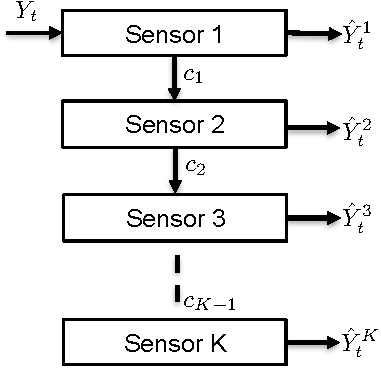
\includegraphics[scale=.5]{SensorCascade.pdf}
	\label{fig:SensorCascade}
	\caption{Cascade of sensors}
\end{figure}


Let $H_t(i)$ denote the feedback observed in round $t$ from action $i$. When the learner selects action $i$ at time $t$, the predictions of all sensors in the selected path are observed and the feedback is $H_t(i)=\{\hat{Y}^1_t,\ldots,\hat{Y}^i_t\}$.
The loss incurred in each round is defined as follows. When the learner selects action $i$, the loss is the error in prediction of sensor $i$ plus the sum of the costs incurred along the path ($c_1,\ldots,c_i$). Let $L_t(i)$ denote the loss in round $t$ for taking action $i$. Then,
\begin{equation}
L_t(i)=\mathbf{1}_{\{\hat{Y}^i_t\neq Y_t\}}+\sum_{j=1}^i c_j.
\end{equation} 
We refer to the above setup as Sensor Acquisition Problem (SAP) and denote it as $\psi=(K,\mathcal{A}, (\gamma_i,c_{i-1})_{i\in [K]})$\footnote{Note that $i\in \mathcal{A}$ implies that action $i$ selects all sensors ${1, 2, \cdots, i}$, not just sensor $i$. We set $c_0=0$}. A policy $\pi=(\pi_1, \pi_2, \cdots)$ on $\psi$, where  $\pi_t : H_{t-1}\rightarrow
\mathcal{A}$, gives action selected in each round using the set of actions played and the corresponding  feedback observed in the past. We compare the performance of policy with respect to the optimal policy (single best action in hindsight) and define expected regret of a policy $\pi$ as follows
\begin{equation}
R^S_T(\pi)= \mathbb{E}\left[\sum_{t=1}^T L_t(a_t)\right]-\min_{i\in A}\mathbb{E}\left[\sum_{t=1}^T L_t(i)\right],
\end{equation}
where $a_t$ denotes the policy selected by $\pi_t$ in round $t$.
The goal of the learner is to learn a policy that minimizes the maximum expected regret, i.e.,
\begin{equation}
\pi^*= \arg \min_{\pi \in \Pi } R_T(\pi)
\end{equation}
where $\Pi$ denote the set of policies that maps past history to an action in $\mathcal{A}$ in each round. 

\noindent
{\bf Optimal action in hindsight: } For any $t$, we have 
\begin{equation}
\mathbb{E}[L_t(k)]=\Pr\{Y_t\neq \hat{Y}^k_t\}+\sum_{j=1}^kc_j=\gamma_k +\sum_{j=1}^kc_j.
\end{equation}
Let $i^*=\arg\min_{i\in \mathcal{A}} \gamma_i + \sum_{j< i}c_j$. Then the optimal policy is to play action $i^*$ in each round. If an action $i$ is played in any round then it adds   $\Delta_i:=\gamma_i + \sum_{j<i}c_j -( \gamma_{i^*} + \sum_{j<i^*}c_i)$. to the expected regret. Let $I_t$ denote the action slected in round $t$ and $N_i(s)$ denote the number of times action $i$ is selected till time $s$, i.e., $N_i(s)=\sum_{t=1}^s \boldsymbol{1}_{\{I_t=i\}}$. Then the expected regret can be expressed as
\begin{eqnarray}
\label{eqn:ExpRegretGap}
R^S_T(\pi)&=& \sum_{i \in \mathcal{A}}\mathbb{E}[N_i(T)]\Delta_i.
\end{eqnarray}\


%\section{Problem Setup}
%\label{sec:Setup}
%We consider the problem of efficient label prediction under partial monitoring. Let $\{Y_t\}_{{t>0}}$ denote sequence of labels generated according to an unknown distribution $\mathcal{D}$.  The learner can use a `cheap' sensor (device-1) or/and a `costly' sensor (device-2) to predict the labels. In round $t$, let $\hat{Y}^1_t$ and $\hat{Y}^2_t$ denote the predictions of device-1 and device-2 respectively. We assume that device-1 has lower performance than device-2 in the sense that prediction error rate of device-1, denoted as 
%$\gamma_1:=\Pr\{Y_t\neq \hat{Y}^1_t\}$, is larger than or equal to that of device-2, denoted as $\gamma_2:=\Pr\{Y_t\neq \hat{Y}^2_t\}$ ($\gamma_1>\gamma_2$). In each round $t$, the learner can take the following actions: 
%\begin{itemize}
%	\item Action-1: use device-1.
% \item Action-2: use both the devices. 
%\end{itemize}
%For ease of notion, we denote actions by their index, and write $\mathcal{A}=\{1,2\}$ for the set of actions and use $i$ to index them. Let $F_t(i)$ denote the feedback observed in round $t$ by selecting action $i$. When $i=1$, the learner observes $\hat{Y}^1_t$, and when $i=2$, he observes both $\hat{Y}^1_t$ and $\hat{Y}^2_t$. That is, 
%\begin{equation}
%F_t(i)=\begin{cases}
%\hat{Y}_t^1 \;\;\mbox{if}\;\;i=1,\\
%\{\hat{Y}^1_t, \hat{Y}^2_t\} \;\;\mbox{if}\;\;i=2.
%\end{cases}
%\end{equation} 
%The loss incurred in each round is defined as follows. When $i=1$, the loss is $1$ unit if prediction of device-1 (observed feedback) is incorrect, otherwise loss is zero. When $i=2$, a fixed loss of $c>0$ is incurred in addition to the prediction loss of device-2, which is $1$ unit if device-2's prediction is incorrect and $0$ otherwise. Let $L_t(i)$ denote the loss in round $t$ for taking action $i\in \mathcal{A}$. Then,
%\begin{equation}
%L_t(i)=\begin{cases}
%\boldsymbol{1}_{\{\hat{Y}^1_t \neq Y_t\}} \;\;\mbox{if}\;\;i=1,\\
%\boldsymbol{1}_{\{\hat{Y}^2_t\neq Y_t\}}+c \;\;\mbox{if}\;\;i=2.
%\end{cases}
%\end{equation} 
%Let $H_{t}$ denote the set of actions played and the corresponding feedback observed till time $t$.  A policy $\pi=(\pi_1, \pi_2, \cdots)$, where  $\pi_t : H_{t-1}\rightarrow
%\mathcal{A}$, gives action selected in each round using all the feedback observed in the past. The expected regret of a policy $\pi$ that selects action $\pi_t \in\mathcal{A}$ in round $t$ over a period $T$ with respect to the best action in hindsight is given as 
%\begin{equation}
%\label{eqn:Regret2Actions}
%R_T(\pi)= \mathbb{E}\left [\sum_{t=1}^TL_t(\pi_t)\right]
%-\min_{i\in \mathcal{A}}\mathbb{E}\left [\sum_{t=1}^T L_t(i)\right ].
%\end{equation}
%The goal of the learner is to learn a policy that minimizes the maximum expected regret, i.e.,
%\begin{equation}
%\pi^*= \arg \min_{\pi \in \Pi }R_T(\pi)  ,
%\end{equation}
%where $\Pi$ denote the set of policies that maps past history to an action in $\mathcal{A}$ in each round. 
%
%\noindent
%{\bf Optimal action in hindsight: } For any $\pi \in \Pi$ and in any round $t$ we have 
%\begin{equation}
%\mathbb{E}[L_t(i)]=
%\begin{cases}
%\gamma_1\;\; \mbox{if}\;\; i=1,\\
%\gamma_2+c\;\; \mbox{if}\;\;i=2,
%\end{cases}
%\end{equation}
%Let  $i^*=\arg\min_{i \in \mathcal{A}} {E}[L_t(i)]$ denote optimal action. Then, $i^*=1$ if $\gamma_1 \leq \gamma_2 +c$, and $i^*=2$ otherwise. Let $I_t$ denote the action taken in round $t$ and $N_i(s)$ denote the number of times action $i$ is selected till time $s$, i.e., $N_i(s)=\sum_{t=1}^s \boldsymbol{1}_{\{I_t=i\}}$. The expected regret can be expressed as
%\begin{eqnarray}
%\label{eqn:ExpRegretGap}
%R_T(\pi)&=& \sum_{i=1}^{2}\mathbb{E}[N_i(T)]\Delta_i 
%\end{eqnarray}
%where $\Delta_1=\gamma_1 -\mathbb{E}[L(i^*)]$ and $
%\Delta_2=\gamma_2+c -\mathbb{E}[L(i^*)]$. Note that for all $i=1,2$, either $\Delta_i=|\gamma_1-\gamma_2-c|$ or $\Delta_i=0$.
%
%
%\noindent
%{\bf Assumptions (Dominance condition):}   Whenever device-1 makes no prediction error, device-2 is also guaranteed to make no prediction error, i.e., in every round $t$, 
%\begin{equation}
%\label{eqn:DomAssum}
%{\hat{Y}^1_t=Y_t} \implies {\hat{Y}^2_t=Y_t}.
%\end{equation}  
%\noindent
%{\bf Reduction to the apple tasting problem:}
%The feedback from action $i=1$ reveals no information about the loss incurred in that round. However feedback after action $i=2$ reveals (partial) information about the loss of both actions. Suppose feedback is such that the predictions of devices disagree, i.e., ${\hat{Y}^1_t\neq\hat{Y}^2_t}$ after action $2$.  The dominance condition then implies that the only possible events are $\hat{Y}^1_t \neq Y_t$ and $\hat{Y}^2_t=Y_t$. I.e., the true label is that predicted by device-2 and loss is zero. Suppose the predictions of the devices agree, i.e., ${\hat{Y}^1_t = \hat{Y}^2_t}$, then the dominance condition implies that either predictions of both are correct or both are incorrect. Though the true loss is not known in this case, the learner can infer some useful knowledge: in round $t$, if the prediction of both the devices agree, then the difference of loss of the actions is $L_t(2)-L_t(1)=c>0$. And if the predictions of the devices disagree, then dominance assumption implies that $L_t(1)=1$ and $L_t(2)=c$ or $L_t(2)-L_t(1)=c-1<0$. Thus, each time learner selects action $2$, he gets to know whether or not he was better off by selecting the other action. This setup is similar the standard apple tasting problem \cite{IC2000_AppleTasting_HelmboldLittlestoneLong}
%], but differs in terms of the information structure when action $2$ is played: in the apple tasting problem, playing action $2$ in a round reveals loss incurred by both the actions. Whereas, in the sensor selection problem we get only partial information on which of the two actions is better in that round. However, we will see below that the partial information is enough to distinguish the optimal arm and one can obtain performance similar to that in the apple tasting problem .

\section{Background on Stochastic Multi-armed Bandits}
A stochastic multi-armed bandit (MAB), denoted as $\phi:=(K, (\nu_k)_{1 \leq k \leq K})$, is a sequential learning problem where number of arms $K$ is known and each arm $k \in [K]$ gives rewards drawn according an unknown distribution $\nu_k$. A policy of the learner is any allocation strategy that selects an arm in each round based on the past history.  Let $X_{i,n}$ denote the random reward from arm $i$ in its $n$th play. For each am $i\in [K]$ $\{X_{i,t}: t>0\}$ are independently and identically (i.i.d) distributed and they are independent across arms. We note that in the standard MAB setting, the learner only observes reward from the selected arm and no information from the other arms is revealed in that round. The performance of a policy is measured with respected to the optimal performance defined in terms of cumulative regret (or simply regret) as follows:  Let $\pi$ denote a policy that selects arm $k_t$ in round $t$. The regret of policy $\pi$ after $T$ rounds is 
\begin{equation}
\label{eqn:BanditRegret}
R^B_T(\pi)= \max_{1\leq i\leq K}\mathbb{E}\left[\sum_{t=1}^{T}X_{i,t}\right]- \mathbb{E}\left[\sum_{i=1}^{T}X_{k_t,N_{k_t}(t)}\right],
\end{equation} 
where $N_{k}(t)=\sum_{s=1}^{t}\boldsymbol{1}\{k_s =k\}$ denotes the number of plays of arm $k$ till round $t$. 
For each $k \in [K]$, let $\mu_k$ denote the mean value distribution $\nu_k$ and $i^*= \arg\min_{i \in [K]} \mu_i$ denote an arm with the smallest mean. The regret of a policy $\pi$ can be expressed 
\[R^B_T(\pi)=\sum_{k=1}^{K}(\mu_{i^*}-\mu_i)\mathbb{E}[N_i(T)].\]
The goal of the learner is to learn a policy that minimizes the regret.  

MAB problems have been extensively studied in the literature. The seminal paper of Lai \& Robbins 
\cite{AAM85_Asymptotically_LaiRobbins} showed that for any consistent policy (that plays sub-optimal arms only sup-polynomially many times in the time horizon) the regret grows logarithmically in time horizon. Specifically, for a class of parametric reward distributions, they showed that regret of consistent policy satisfies
\begin{equation}
\label{eqn:MABLowerBound}
\liminf_{n \rightarrow \infty}\frac{ R^B_T(\pi)}{\log T} \geq \sum_{i\neq i^*} \frac{\mu_{i^*}-\mu_i}{D(\mu_{i^*}||\mu_i)},
\end{equation}
where  $D(p||q)$ denote the KL-divergence of $p,q \in [0\; 1]$. Further, the authors in \cite{AAM85_Asymptotically_LaiRobbins}  provided an upper confidence bound (UCB) based policy that asymptotically achieves the lower bound for a class of parmetric reward distributions.
 
Auer et, al. \cite{ML02_FiniteTimeAnalysis_AuerBianchiFischer} proposed an anytime policy named UCB1 that is based on the UCB strategy and showed that it is optimal on any MAB with bounded rewards. Specifically, they showed that regret of UCB1 for any $T>K$ is upper bound as 
\begin{equation}
\label{eqn:UCB1UpperBound}
R^B_T(UCB1)\leq \sum_{i\neq i^*} \frac{8\log n}{\mu_{i^*}-\mu_i} + (\pi^2/3 + 1)(\mu_{i^*}-\mu_i).
\end{equation}
Thus demonstrating the optimality of UCB1. Since the work of Auer et. al. several works have proposed improvised UCB based policies like, KL-UCB, MOSS.


\subsection{MAB With Side Information}
In many applications playing an arm reveals information about the other arms which can be exploited to improve learning performance. Let $\mathcal{N}_i$  denote the set of arms such that playing arm $i$ reveals rewards of all arms $j \in \mathcal{N}_i$. We refer to $\mathcal{N}_i$ as neighborhood of $i$ and the graph induced by the neighborhood sets as side-information graph. Given a set of neighborhood $\{\mathcal{N}_i, i\in [K]\}$, let $\phi_G:=(K, (\nu_k)_{1\leq k\leq K}, G)$ denote a MAB with side-information graph $G=(V,E)$, where $|V|=K$ and $(i,j)\in E$ if $j \in \mathcal{K}_i$.The side-observation graph is known to the learner and remains fixed during the play. 

A policy for $\phi_G$ maps the past history (including the side-observations) to an action in each round. With some abuse of notation, we denote the regret of any policy $\pi_G$ that uses side-information over a period $T$ as $R^B_T(\pi_G)$ and is given by (\ref{eqn:BanditRegret}). Note that, in each round, 
only reward from the arm played contribute to the regret and not that from the side-observations. In \cite{Sigmetrics15_StochasticBanditsWithSideObservations_BuccapatnamEriyilmazShroff} the authors extended the lower bound in (\ref{eqn:MABLowerBound}) to incorporate the effect of side-observations. Specifically, they established that any policy $\pi_G$ on a graph where $i \in \mathcal{N}_i$ for all $i\in [K]$ satisfies
%\begin{equation}
%\label{RegretBandit}
%R^B_T(\pi)= \max_{1\leq i\leq K}\mathbb{E}\left[\sum_{t=1}^{T}X_{i,t}\right]- \mathbb{E}\left[\sum_{i=1}^{T}X_{k_t,N_{k_t}(t)}\right],
%\end{equation} 
 \cite{Sigmetrics15_StochasticBanditsWithSideObservations_BuccapatnamEriyilmazShroff}

\begin{equation}
	\liminf_{T \rightarrow \infty} R^B_T(\pi_G)/\log T \geq \eta(G)
	\end{equation}
	where $\eta(G)$ is the optimal value of the following linear program
	\begin{align}
	& LP1: \;\displaystyle\min_{\{w_i\}}\sum_{i \in [K]}(\mu_{i^*}- \mu_i) w_i \nonumber\\
	\label{eqn:LowerBoundLP}
	& \mbox{subjected to} \sum_{j \in \mathcal{N}_i}w_i\geq 1/D(\mu_i || \mu_{i^*}) \mbox{  for all } i\in [K]\\
	& w_i \geq 0 \mbox{ for all } i \in [K] \nonumber
	\end{align}
	
\begin{definition}[Domination number \cite{Sigmetrics15_StochasticBanditsWithSideObservations_BuccapatnamEriyilmazShroff}]
	Given a graph $G=(V,E)$, a subset $W\subset V$ is a dominant set if for each $v\in V$ there exists $u \in W$ such that $(u,v)\in E$. The size of the smallest dominant set is called weak domination number and denoted as $\xi(G)$. 
\end{definition} 	
	
The authors in \cite{Sigmetrics15_StochasticBanditsWithSideObservations_BuccapatnamEriyilmazShroff} gave an UCB based strategy, named UCB-LP, that exploits the side-observations structure and explore arms at a rate in proportion to the size of their neighborhood. UCB-LP plays arms in proportions to the values $\{z_i^*, i\in [K]\}$ computed from the following linear programmer which is a relaxation of linear programme $LP1$. 
	\begin{align}
	& LP2: \displaystyle\min_{\{z_i\}}\sum_{i \in [K]} z_i \nonumber\\
	\label{eqn:LowerRelaxedBoundLP}
	& \mbox{subjected to} \sum_{j \in \mathcal{N}_i}z_i\geq 1 \mbox{  for all } i\in [K]\\
	& z_i \geq 0 \mbox{ for all } i \in [K] \nonumber
	\end{align}
The regret of UCB-LP is upper bounded by 
\begin{equation}
\label{eqn:UCBLPUpperBound}
\mathcal{O}\left(\sum_{i\in [K]} z_i^* \log T\right) +\mathcal{O}(K\delta),
\end{equation}
where $\delta= \max_{i \in [K]}|\mathcal{K}_i|$ and $\{z_i^*\}$ are the optimal values of $LP2$. Since any dominating set is a feasible solution of $LP2$, we get $\sum_{i\in [K]}z_i^*\leq \xi(G)$, and the regret of UCB-LP is $\mathcal{O}(\xi(G)\log T)$. 
\subsection{Special case: 1-armed bandit}
In the MAB problem when all the arms have a fixed reward except for one, we get 1-armed bandit. 
The learner knows the arms that give fixed reward the goal is to identify the quality of the arm that gives stochastic reward as fast as possible. A straightforward modification of UCB1 achieves optimal regret of $\Theta(\log T)$.
  
 \section{Regret Equivalence}
In the SAP, the true labels are never revealed, hence the learner cannot learn the error rates of the sensors. Thus, SAP appears to be an hopeless case where nothing can be learned. In this section we establish that seemingly hopeless SAP can be efficiently solved provided the following dominance condition holds:

\begin{assumption}[Dominance Condition]
If sensor $i$ predicts correctly, all the sensors in the subsequent stages of the cascade also predict correctly, i.e.,
 
\begin{equation}
\label{eqn:DominanceCondition}
\hat{Y}_t^i=Y_t \rightarrow \hat{Y}_t^j \quad \forall j>i\geq 1
\end{equation}
\end{assumption}
\noindent
In the following we establish that under the dominance condition SAP is `regret equivalent' to an instance of MAB with side-information and the corresponding algorithm for MAB can be suitably imported to solve SAP efficiently.   
 \noindent
\begin{definition}[Regret Equivalence]
	Consider a SAP problem $\psi:=(K, \mathcal{A}, (\gamma_i,c_{i-1})_{i\in [K]})$ and a bandit problem with $\phi_G:=(N, (\nu_i)_{i \in [N]},G)$ side-information graph $G$. We say that $\psi$ is regret-equivalent to $\phi_G$ if given a policy $\pi$ for problem $\psi$, one can come up with a policy $\pi^\prime$ that uses $\pi$, such that the regret of $\pi^\prime$ on any instance of $\phi_G$ is the same as the regret of $\pi$ on some corresponding instance of $\psi$, and vice versa. 
\end{definition}	
In the following we first consider the SAP with 2 sensors and then the general case with more than 2 sensors. The 2 sensors case helps to draw comparison with the well studied apple tasting problem and understand role of the dominance condition. 
\subsection{SAP with two sensors}
In the SAP with only two actions, the feedback from action $i=1$ reveals no information about the loss incurred in that round. However feedback after action $i=2$ reveals (partial) information about the loss of both actions. Suppose feedback is such that predictions of the sensors disagree, i.e., ${\hat{Y}^1_t\neq\hat{Y}^2_t}$ after action $2$.  The dominance condition then implies that the only possible events are $\hat{Y}^1_t \neq Y_t$ and $\hat{Y}^2_t=Y_t$. I.e., the true label is that predicted by sensor-2, hence loss incurred is just $c$ (prediction loss is zero). Suppose predictions of the sensors agree, i.e., ${\hat{Y}^1_t = \hat{Y}^2_t}$, then the dominance condition implies that either predictions of both are correct or both are incorrect. Though the true loss is not known in this case, the learner can infer some useful knowledge: in round $t$, if prediction of both the sensors agree, then the difference in losses of the actions is $L_t(2)-L_t(1)=c>0$. And if predictions of the sensors disagree, then dominance assumption implies that $L_t(1)=1$ and $L_t(2)=c$ or $L_t(2)-L_t(1)=c-1<0$. Thus, each time learner plays action $2$, he gets to know whether or not he was better off by selecting the other action. This setup sounds similar to the standard apple tasting problem \cite{IC2000_AppleTasting_HelmboldLittlestoneLong}
], but differs in terms of the information structure when action $2$ is played. 

\noindent
{\bf Apple tasting problem:} In the apple tasting problem, a learner gets a sequence of apples and some of them can be rotten. In each round, the learner can either accept or reject an apple. If an apple is accepted, the learner tastes it and incurs a penalty if it is rotten. If apple is rejectsed, he still incurs the penalty if it is rotten, but do not get to observe its quality. %Thus, each time the learner accepts an apple, he knows the penalty incurred for both the actions. However, no loss values is revealed if he rejects. 
The goal of the learner is to taste more good apples. 
The SAP setting is a more general version than the apple tasting problem--in any round, actions $1$ reveals no loss values. Action $2$  reveals only partial information about the losses, but not the exact losses as in the apple tasting problem. However, we next show that the partial information is enough to achieve optimal performance.  

\begin{thm}
	\label{thm:SATRegret}
Assume dominance condition (\ref{eqn:DominanceCondition}) holds. Then SAP $\psi$ with $K=2$ is regret-equivalent to a stochastic $1$-armed bandit.
\end{thm}
{\bf Proof:}
Consider a $1$-armed stochastic bandit problem where arm with constant reward has value $c$ and the arm that gives stochastic reward has mean value  $\gamma_1-\gamma_2$.  
Given an arbitrary policy $\pi=(\pi_1, \pi_2, \cdots \pi_t )$ for the SAP, we obtain a policy for the bandit problem from $\pi$ as follows: Let $H_{t-1}$ denote the history, consisting of all arms played and the corresponding rewards, available to policy $\pi_{t-1}$ till time $t-2$. Let $a_{t-1}$ denote the action selected by the bandit policy  in round $t-1$ and $r_{t-1}$ the observed reward. Then, the next action $a_t$ is obtained as follows:
\begin{equation}
\label{eqn:SAPto1Bandit}
a_t=
\begin{cases}
\pi_t(H_{t-1}\cup \{1, \emptyset
 \}) \mbox{ if } a_{t-1}= \mbox{fixed rewad arm}	\\
 \pi_t(H_{t-1} \cup \{2, r_{t-1}\}) \mbox{ if } a_{t-1}= \mbox{stochastic arm}
\end{cases}
\end{equation}
\noindent
Conversely, let $\pi^\prime=\{\pi^\prime_1, \pi^\prime_2,\cdots\}$ denote an arbitrary policy for the 1-armed bandit problem. we obtain a policy for the SAP as follows: Let $H^\prime_{t-1}$ denote the history, consisting of all actions played and feedback, available to policy $\pi^\prime_{t-1}$ till time $t-1$. Let $a^\prime_{t-1}$ denote the action selected by the SAP policy in round $t-1$ and observed feedback $F_t$. Then, the next action $a^\prime_t$ is obtained as follows:
\begin{equation}
\label{eqn:1BanditToSAP}
a^\prime_t=
\begin{cases}
\pi^\prime_t(H^\prime_{t-1} \cup \{1, c
\}) \mbox{ if } a^\prime_{t-1}= \mbox{action 1}	\\
\pi^\prime_t(H^\prime_{t-1} \cup \{2, \boldsymbol{1}\{\hat{Y}_t^1\neq \hat{Y}_t^2\}\}) \mbox{ if } a_{t-1}= \mbox{actions 2}.
\end{cases}
\end{equation}
We next show that regret of $\pi$ on the SAP is same as that of derived policy on the 1-armed bandit, and  regret of $\pi^\prime$ on the 1-armed bandit is same as regret of the derived policy on SAP. 
We first argue that any policy on the SAP problem with 2 actions needs the information if whether the predictions of sensors match or not whenever action $2$ is played.  The following observation is straightforward.
\begin{lemma}
	\label{lma:SuffStat2Action}
	Let  dominance condition holds. Then, $\Pr\{\hat{Y}^1_t \neq \hat{Y}^2_t\}=\gamma_1-\gamma_2$.
\end{lemma}
\begin{eqnarray}
\lefteqn{\Pr\{\hat{Y}^1_t \neq \hat{Y}^1_t\}=\Pr\{\hat{Y}^1_t=Y_t, \hat{Y}^2_t \neq Y_t\} + \Pr\{\hat{Y}^2_t=Y_t, \hat{Y}^1_t \neq Y_t\}} \\
&=& \Pr\{\hat{Y}^2_t=Y_t, \hat{Y}^1_t \neq Y_t\} \;\;\mbox{from assumption (\ref{eqn:DominanceCondition})}\\
&=& \Pr\{\hat{Y}^1_t\neq y_t\}\Pr\{\hat{Y}^2_t= Y_t| \hat{Y}^1_t\neq Y_t\} \\
&=& \Pr\{\hat{Y}^1_t\neq Y_t\}\left( 1-\Pr\{\hat{Y}^2_t \neq  Y_t| \hat{Y}^1_t\neq Y_t\} \right ) \\
&=& \Pr\{\hat{Y}^1_t\neq Y_t\}\left( 1-\frac{\Pr\{\hat{Y}^2_t \neq  Y_t, \hat{Y}^1_t\neq Y_t\}}{\Pr\{\hat{Y}^1_t\neq Y_t\}} \right )\\
&=& \Pr\{\hat{Y}^1_t\neq Y_t\}-\Pr\{\hat{Y}^2_t \neq  Y_t\}  \;\; \mbox{by contrapositve of  (\ref{eqn:DominanceCondition})} 
\end{eqnarray}
From Lemma \ref{lma:SuffStat2Action}, mean of the observations $Z_t:=\boldsymbol{1}{\{\hat{Y}_t^1 \neq \hat{Y}_t^2 \}}$ from action $2$ in the SAP is a sufficient statistics to identify the optimal arm. Thus, any SAP only needs to know $Z_t$ in each round, and $Z_t$ are i.i.d with mean $\gamma_1-\gamma_2$.  Our mapping of policies is such that any poilcy for SAP (1-armed bandits) and the derived policy on the 1-armed bandit (SAP) play the sub-optimal arm same number of times.  For the sake of simplicity assume that action $1$ is optimal for SAP  $(\gamma_1> \gamma_2 + c)$ and let a policy $\pi$ on SAP plays it $N_1(T)$ number if times. Then, we have
\[ R^S_T(\pi)=\Delta_i\mathbb{E}[N_1(T)]=(\gamma_1-\gamma_2-c)\mathbb{E}[N_1(T)]\]
Let $f(\pi)$ denote the policy for the 1-armed bandit obtained using the mapping (\ref{eqn:SAPto1Bandit}). Now, for the $1$-armed bandit, where the arm with stochastic rewards is optimal, we have
\[ R^B_T(f(\pi))=(\mu_2-\mu_1)\mathbb{E}[N_1(T)]=(\gamma_1-\gamma_2-c)\mathbb{E}[N_1(T)]\]
Thus the regret of $\pi$ on the SAP problem and that of $f(\pi)$ on the $1$-armed bandit are the same. We can argue similarly for the other cases. 
%a_i\mathbb{E}[N_i(T)]$ where $\Delta_1= c- \min\{\gamma_1-\gamma_2,c\}$ and $\Delta_2= \gamma_1-\gamma_2- \min\{\gamma_1-\gamma_2,c\}$, which can also be expressed as $\Delta_1=\gamma_1 - \mathbb{E}[L(i^*)]$ and  $\Delta_2=\gamma_2+c - \mathbb{E}[L(i^*)]$, implying that the corresponding policy on the SAP also gives the same regret and vice versa. 
The following corollary follow immediately from the regret equivalence. 
\begin{proposition}[SAP regret lower bound]
	Let $\pi$ be any policy on SAT with 2 sensors such that it pulls the suboptimal arm only sub polynomial many times, i.e., $\mathbb{E}[N_i(T)]=o(T^a)$ for all $a>0$ and $i\neq i^*$. Then,
	\begin{equation}
	\liminf_{T \rightarrow \infty} R^S_T(\pi)/\log T \geq \frac{|\gamma_1-\gamma_2-c|}{D(\gamma_1-\gamma_2,c)}
	\end{equation}
	where $D(\gamma_1-\gamma_2,c)$ is the KL-divergence between $\gamma_1-\gamma_2$ and $c$.
\end{proposition}

\begin{proposition}[SAT regret upper bound]
	Let $\pi^\prime$ denote a policy on a $1$-armed stochastic bandit where one arm has mean $\gamma_1-\gamma_2$ and the other gives fixed reward $c$. Then, the regret of a policy $g(\pi)$ for the SAT problem obtained according the mapping (\ref{eqn:1BanditToSAP}) is upper bounded as
	\begin{equation}
	R^S_T(g(\pi))\leq \frac{6\log T}{|\gamma_1-\gamma_2-c|} + |\gamma_1-\gamma_2-c|(1+\pi^2/3)
	\end{equation}
	when $\pi^\prime=UCB1$
\end{proposition}
\subsection{SAP with more than two actions}
In the SAP with two sensors, only action 2 provides information about the losses. In the case with $K>2$ sensors, by applying the dominance condition recursively to any pair of actions we can obtain information about the losses for all actions $i>2$. Further, any information provided by action $i>2$ is contained in that provided by all actions $j\geq i$. If action $i$ is played in round $t$, then we observe predictions $\{\hat{Y}_t^1, \hat{Y}_t^2, \cdots, \hat{Y}_t^i\}$ which includes the observed predictions for all actions $j\leq i$. Hence, action $i$ provides information about all actions $j\leq i$ This side-observation can be represented by a directed graph $G^S=(V,E)$, where $|V|=K$ and $E=\{(i,j): i 1<i\leq j\leq K \}$. Note that $G^S$ has self loops for all nodes except for node $1$. The nodes in $G^S$ represents actions of the SAP and an edge $(i,j)\in E$ implies that actions $i$ provides information about action $j$. The side-observation graph for the SAP is shown in Figure (\ref{fig:SideObservationGraph]}).

\begin{figure}[!h]
	\centering
	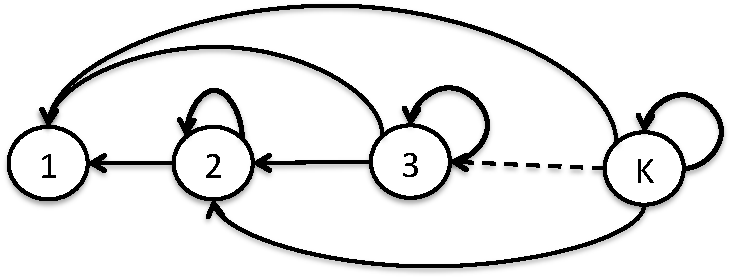
\includegraphics[scale=.5]{SideInfoGraph.pdf}
	\caption{Side observation graph $G^S$}
	\label{fig:SideObservationGraph]}
\end{figure}  
\begin{thm}
Let the dominance condition (\ref{eqn:DominanceCondition}) holds. Then SAP $\psi$ with $K\geq 2$ is regret equivalent to a MAB with side-observation graph $G^S$. 
\end{thm}

Consider a $K$-armed stochastic bandit problem where rewards distribution $\nu_i$ has mean  $\gamma_1-\gamma_i- \sum_{j< i}c_j$ for all $i >1$ and arm $1$ gives a fixed reward of value $0$. The arms have side-observation structure defined by graph $G^S$.  
Given an arbitrary policy $\pi=(\pi_1, \pi_2, \cdots \pi_t )$ for the SAP, we obtain a policy for the bandit problem with side observation graph $G^S$ from $\pi$ as follows: Let $H_{t-1}$ denote the history, consisting of all arms played and the corresponding rewards, available to policy $\pi_{t-1}$ till time $t-2$. In round $t-1$, let $a_{t-1}$ denote the arm selected by the bandit policy,  $r_{t-1}$ the corresponding reward and $o_{t-1}$ the side-observation defined by graph $G_S$ excluding that from the first arm. Then, the next action $a_t$ is obtained as follows:
\begin{equation}
\label{eqn:SAPtoKBandit}
a_t=
\begin{cases}
\pi_t(H_{t-1}\cup \{1, \emptyset
\}) \mbox{ if } a_{t-1}= \mbox{arm 1}	\\
\pi_t(H_{t-1} \cup \{i, r_{t-1}\cup o_{t-1}\}) \mbox{ if } a_{t-1}= \mbox{arm i}
\end{cases}
\end{equation}
\noindent
Conversely, let $\pi^\prime=\{\pi^\prime_1, \pi^\prime_2,\cdots\}$ denote an arbitrary policy for the $K$-armed bandit problem with side-observation graph. we obtain a policy the SAP as follows: Let $H^\prime_{t-1}$ denote the history, consisting of all actions played and feedback, available to policy $\pi^\prime_{t-1}$ till time $t-2$. Let $a^\prime_{t-1}$ denote the action selected by the SAP policy in round $t-1$ and observed feedback $F_t$. Then, the next action $a^\prime_t$ is obtained as follows:
\begin{equation}
\label{eqn:KBanditToSAP}
a^\prime_t=
\begin{cases}
\pi^\prime_t(H^\prime_{t-1} \cup \{1, 0
\}) \mbox{ if } a^\prime_{t-1}= \mbox{action 1}	\\
\pi^\prime_t(H^\prime_{t-1} \cup \{i, \boldsymbol{1}\{\hat{Y}_t^1\neq \hat{Y}_t^2\}\cdots \boldsymbol{1}\{\hat{Y}_t^1\neq \hat{Y}_t^i\}\}) \mbox{ if } a_{t-1}= \mbox{action i}.
\end{cases}
\end{equation}
We next show that regret of a policy $\pi$ on the SAP problem is same as that of the policy derived from it for the $K$-armed bandit problem with side information graph $G^S$, 
and regret of $\pi^\prime$ on the $K$-armed bandit with side information graph  $G^S$ is same as that of the policy derived from it for the SAP.

Given a policy $\pi$ for the SAP problem let $f_1(\pi)$ denote the policy obtained by the mapping defined in (\ref{eqn:SAPtoKBandit}). The regret of policy $\pi$ that plays actions $i$, $N_i(T)$ times is given by 
\begin{eqnarray}
R^S_T(\pi) &=&\sum_{i=1}^{K}\left [ \left (\gamma_{i}+\sum_{j< i} c_j\right )-\left (\gamma_{i^*}+\sum_{j < i^*} c_j\right )\right ]\mathbb{E}[N_i(T)]\\
\end{eqnarray}
Now, regret of regret policy $f_1(\pi)$ on the $K$-armed bandit problem with side information graph $G^s$ 
\begin{equation}
R^B_T(f_1(\pi))=\sum_{i=1}^{K} \left[\left (\gamma_1-\gamma_{i^*}-\sum_{j <i^*} c_j \right )-\left (\gamma_1- \gamma_{i}-\sum_{j < i} c_j \right )\right ]\mathbb{E}[N_i(T)]
\end{equation}
which is same as $R^B_T(\pi)$. This concludes the proofs. 
\begin{remark}
Note that the some of mean 	values $\{\gamma_1- \gamma_i - \sum_{j\leq i} c_j\}$ need not be positive. Since the stochastic bandit algorithms assume that reward lie in the interval $[0,1]$, they may not be directly applicable to our setting. However, this can be over come by setting the distributions of arm $k$, $\nu_k$, to have mean $\gamma_1- \gamma_i - \sum_{j< i} c_j + \sum_{k \leq K-1 }c_k$. Note that we translated the mean of each arm by the same amount, which does not change the regret value. For $k=2$, this recovers the SAP with  actions and Theorem \ref{thm:SATRegret} holds
\end{remark}



\begin{proposition}[SAP regret lower bound]
	Let $\pi$ be any policy on SAT with 2 sensors such that it pulls the suboptimal arm only sub polynomial many times, i.e., $\mathbb{E}[N_i(T)]=o(T^a)$ for all $a>0$ and $i\neq i^*$. Then,
	\begin{equation}
	\liminf_{T \rightarrow \infty} R^S_T(\pi)/\log T \geq \kappa
	\end{equation}
	where 
	\begin{align}
	\kappa=&\displaystyle\min_{\{w_i\}}\sum_{i \in [K]}(\mu_{i^*}- \mu_i) w_i \nonumber\\
	& \mbox{subjected to} \sum_{j i}w_i\geq 1/D(\mu_i + \sum_{j<i} c_j || \mu_{i^*}) \mbox{  for all } i\in [K]\\
	& w_i \geq 0 \mbox{ for all } i \in [K] \nonumber
	\end{align}
\end{proposition}

\begin{proposition}[K-SAT regret upper bound]
	Let $\pi^\prime$ denote a policy on a $K$-armed stochastic bandit where mean of arm $i>1$ is $\gamma_1-\gamma_i-\sum_{j<i}c_j$ and arm has a fixed reward of value zero, and the side-observation graph is $G^S$.  Then, the regret of a policy $g_1(\pi)$ for the SAT problem obtained from mapping (\ref{eqn:KBanditToSAP}) is upper bounded as
	\begin{equation}
	R^S_T(g(\pi))\leq \mathcal{O}(\xi(G^S)\log T)
	\end{equation}
	when $\pi^\prime=UCB-LP$ \cite{Sigmetrics15_StochasticBanditsWithSideObservations_BuccapatnamEriyilmazShroff}.
\end{proposition}




%
%\section{Extension to Multi-Stage and Multi-Action setting}
% 
% \subsection{Information and Side Observations:}
% on the feedback observed, we continue to assume that the dominance condition holds across the stages, i.e., for all $1\leq i\leq K-1$
% \begin{equation}
% \label{eqn:DominanceMultiStage}
%\mbox{ if } \hat{Y}_t^i=Y_t  \implies  \hat{Y}_t^j=Y_t \mbox{ for all } i<j\leq K
% \end{equation}
% Then, each time action $i>1$ is played, we get the same type of information about the loss incurred by an action pair  $(j,j-1)$ as in the SAP problem using the pair  $\{\hat{Y}_t^j,\hat{Y}_t^{j-1}\}$ for each $1<j<i$. Thus, playing action $i>1$ provides side observations about all the actions $j\leq ii$. We refer to this setting as Multi stage Sensor Acquisition Problem (MSAP). 
% 
% The side-observation structure in the MSAP problem can be represented by a directed graph $G=(\mathcal{V}, \mathcal{E})$ where $|\mathcal{V}|=K$ and $\mathcal{E}=\{(i,j) \in \mathcal{V}\times \mathcal{V}: i\geq j, i>1\}$. Here,  $(i,j)\in \mathcal{E}$ implies that selecting $i$ provides information about the prediction loss of action $j$. The side-observation graphs is depicted in Figure (\ref{fig:SideObservationGraph]}). Note that an edge $(i,j) \in \mathcal{E}$ only implies that playing action $i$ provides some information about the losses of actions $i\leq j$, but not their true losses. In the following we establish that regret of MSAP is equivalent to a stochastic $K$-armed bandit with the same side-observation structure.
%  \subsection{Regret Equivalence}
% \begin{thm}
% 	A MSAP $(K, \mathcal{A}, (\gamma_i,c_i)_{i\in [K]}, (L(i), F(i))_{i \in \mathcal{A}} )$ with $K>2$ is regret-equivalent to a stochastic bandit problem $(N, (\nu_i)_{i \in [N]})$ with $N=K$ and side observation structure give by $G$.
% \end{thm}	
%Consider a $K$-armed stochastic bandit problem where  reward distribution $\nu_k$ has mean $\gamma_1-\gamma_k + \sum_{j=2}^k c_j$ for all $1\leq k\leq K$, and the side-observation from arms is given by graphs $G$ . Given an arbitrary policy $\pi$ for the MSAP  that uses the side-information, we obtain a  policy BanditG($\pi$) for the bandit problem as follows: if BanditG($\pi$) played arm $i\neq 1$ in the previous round, it inputs the feedback observed from all arms $i\leq j$ to $\pi$ and copies $\pi$'s choice for next action. If BanditG($\pi$)  played arm $1$ in the previous round, it simply copies $\pi$'s choice for next action. Conversely, suppose $\theta$ is an arbitrary policy for the bandit problem with side-observation structure $G$, let MSAP($\theta$) denote a policy for MSAP that consults $\theta$ as follows: if MSAP($\theta$) played action $i$ in the previous round it inputs feedback vector $(0, \boldsymbol{1}_{\{\hat{Y}_t^j\neq \hat{Y}_t^{j-1} \}}, \forall \; j\leq 1)$ to $\theta$ and copies its choice for next action. Otherwise it simply copies $\theta$'s choice for next action.
%
%We next show that regret of BanditG($\pi$) on the bandit problem is same as that of $\pi$ on MSAP, 
% and regret of MSAP($\theta$) on MSAP is same as regret of $\theta$ on the bandit problem. 
% 
%For any strategy $\pi$, the expected regret of the MSAP can be expressed as 
%\begin{eqnarray}
%R_T(\pi) &=&\sum_{i=1}^{K}\left [ \left (\gamma_{i}+\sum_{j\leq i} c_j\right )-\left (\gamma_{i^*}+\sum_{j\leq i^*} c_j\right )\right ]\mathbb{E}[N_i(T)]\\
%&=&\sum_{i=1}^{K} \left[\left (\gamma_1+c_1-\gamma_{i^*}-\sum_{j\leq i^*} c_j \right )-\left (\gamma_1+c_1- \gamma_{i}-\sum_{j\leq i} c_j \right )\right ]\mathbb{E}[N_i(T)]
%\end{eqnarray} 
%where we added and subtracted $\gamma_1+c_1$ from each term. Now, notice that this is the expected regret of the policy on a stochastic bandit where the mean rewards  are 
%\begin{equation}
%\gamma_1+c_1 - \gamma_i - \sum_{j\leq i} c_j \quad \mbox{for } i=1,2,\cdots, K. 
%\end{equation}
%\begin{remark}
%Note that the some of mean 	values $\gamma_1+c_1 - \gamma_i - \sum_{j\leq i} c_j$ need not be positive. Since most of the stochastic bandit algorithms assume that reward lie in the interval $[0,1]$, they may not be directly applicable to our setting. However, this can be over come by setting the distributions of arm $k$, $\nu_k$, to have mean $\gamma_1+c_1 - \gamma_i - \sum_{j\leq i} c_j + \sum_{k=2}^K c_k$. Note that we translated the mean of each arm by the same amount this does not change the regret value. For $k=2$, this recovers the SAT problem and Theorem \ref{thm:SATRegret} holds
%\end{remark}
%$\wedge$
%
%\begin{thm}[Upper Bound]
%	
%\end{thm}
%\begin{thm}
%	
%\end{thm}
%When we pull an arm  $i$, we observe a realization of a distribution with mean $\gamma_1 -\gamma_i$, but since the cost values are fixed, this is equivalent to observe realization of a distribution with mean $\gamma_1 +c_1-\gamma_i + \sum_{j\leq i}c_i$. Thus, the sensor selection problem with mean costs $\{\gamma_i + \sum_{j\leq i}c_i\}$ is equivalent to a stochastic multi-armed problem with mean rewards $\{\gamma_1+c_1 -\gamma_i - \sum_{j\leq i}c_i\}$. 

% \alglanguage{pseudocode}
% \begin{algorithm}[!h]
% 	\footnotesize
% 	\caption{StAT-K}
% 	\label{Algorithm:Stochastic Apple Tasting1}
% 	\begin{algorithmic}[1]
% 		\State \textbf{Input:}
% 		\State $c_k$ cost of sensor $k=2\cdots,K $
% 		\State \textbf{Initialization:}
% 		\State Play $a_K$ once, observe $X_{j,t}^i$, for all $K \geq j>i\geq 1$
% 		\State $N_{K}(1)\leftarrow 1 $, $Y_{j,1}^i\leftarrow X_{j,1}^i$ and $\hat{\mu}_{j,1}^i\leftarrow \frac{Y_{j,1}^i}{N_{K}(1)}$ for all $K \geq j > i\geq 1$
% 		\For {$t = 2,3\cdots$}
% 		\State {\bf Select the best action optimistically. How? We can use pairwise information to select the best action as follows}  
% 		\For {$j=2,3,\cdots, K$}
% 		\State $I\leftarrow 1$
% 		\If {$\hat{\mu}_{j,t-1}^I + \sqrt{\frac{6\log t}{\sum_{k\geq j} N_{k}(t-1)}} > \displaystyle \sum_{k=I+1}^{j}c_k$}  \quad //Checks if action $I$ is better than action $i$,
% 		\State $I\leftarrow j$
% 		\Else
% 		\State $I \leftarrow I$
% 		\EndIf
% 		\EndFor
% 			\State play action $a_I$ and observe $X_{I,t}^i$ for all $I>i\geq 1$,
% 			\State $N_{I}(t) \leftarrow N_{I}(t-1)+1$, $Y_{I,t}^i\leftarrow Y_{I,t-1}^j+X_{I,t}^i$ for all $ I>i \geq 1$
% 			\State $\hat{\mu}_{I,t}^i \leftarrow \frac{Y_{I,t}^i}{\sum_{k=I}^{K}N_k(t)}$ for all $ I>i \geq 1$
% 		\EndFor 
% 		
% 		\Statex
% 	\end{algorithmic}
% 	% \vspace{-0.4cm}%
% \end{algorithm}
% 
%
%\section{Algorithm}
%Let $X_{j,t}^i=\boldsymbol{1}_{\{\hat{y}^{i}_t \neq \hat{y}^j_t\}}, j>i$ denote whether the predictions of sensors $i$ and $j$ agree or not in round $t$. Note that $X_{j,t}^i$ is observed whenever learner selects action $a_k, k>j$. Let $\hat{\mu}_{j,t}^i$ denote the empirical mean of the samples $\{X_{j,t}^t\}$ observed till time $s$, given by
%\begin{equation}
%\hat{\mu}_{j,s}^i= \frac{\sum_{t=1}^s X_{j,t}^i\boldsymbol{1}_{\{I_t\geq j\}}}{\sum_{k=j}^{K}N_k(s)}.
%\end{equation}
%
%
%{\bf Remarks: We discussed the strategy in Algorithm-1 (StAT-K). Consider the case of perfect knowledge of $\gamma_i$'s and assume $j^{th}$ action is optimal. Then we know that $\gamma_i - \gamma_j> \sum_{k=i+1}^{j} c_k$ for all $i<j$ and $\gamma_j - \gamma_i < \sum_{k=j+1}^{i} c_k$ for $j<i$. However, after estimating the $\gamma_i$'s and selecting the best action optimistically as in StAT-K does not lead to similar argument, i.e.,  suppose in round $t$, $I^{th}$ action is selected by StAT-K, then the following need not hold.}
%
%\[{\hat{\mu}_{I,t-1}^j + \sqrt{\frac{6\log t}{\sum_{k\geq I} N_{k}(t-1)}} > \displaystyle \sum_{k=j}^{I}c_k} \quad for \;\;  I>j\]
%and
%
%\[{\hat{\mu}_{j,t-1}^I + \sqrt{\frac{6\log t}{\sum_{k\geq j} N_{k}(t-1)}} < \displaystyle \sum_{k=I+1}^{j}c_k} \quad for \;\; j> I\]
%

\section{Extension to context based prediction}
In this section we consider that learner gets contextual information. Let $x_t \in \mathcal{C}\subset\mathcal{R}^d$ denote the context associated with $y_t$, where $\mathcal{C}$ denotes a compact set. 

Let $L_t(a|x)$ denote the loss incurred by selecting action $a$ when the context is $x$. For any policy $\pi:\mathcal{C}\rightarrow \mathcal{A}$, let $\pi(x_t)$ denote the action selected when the context is $x_t$ using the observed feedback from past actions. For any sequence fo samples ${x_t,y_t}_{t>0}$, the regret of a policy $\pi$ is defined as:
\begin{equation}
R_T(\pi)= \sum_{t=1}^{T} (L_t(\pi(x_t))-L_t(a^*(x_t)))
\end{equation}
where $a^*(x)=\arg \min_{a\in \mathcal{A}}\mathbb{E}[L_t(a|x)]$. The goal is to learn a policy that minimizes the expected regret, i.e.,
\begin{equation}
\pi^*= \arg \min_{\pi \in \Pi} \mathbb{E}[R_T(\pi)].
\end{equation}
We first consider the case with two actions studied in Section \ref{sec:Setup}. The predictions of both the devices are context dependent denoted as $\gamma_1(x_t)=\Pr\{\hat{y}^1_t\neq y_t|x_t\}$ and $\gamma_1(x_t)=\Pr\{\hat{y}^2_t\neq y_t|x_t\}$.  We assume that the difference of prediction errors satisfy  $\gamma_1(x)-\gamma_2(x)=\theta^\prime x$ for all $x \in \mathcal{C}$ for some $\theta \in \mathcal{R}^d$.
\section{Relaxing the dominance assumption}
We next consider weaker dominance condition. Suppose we interpret label-1 as `threat', it is natural to assume that whenever device-2 does not label incoming instance as threat, then device-1 also does the same. Specifically, we assume that 
\begin{equation}
	{\hat{y}^2_t \neq 1} \implies {\hat{y}^1_t \neq 1},
\end{equation}
which is equivalent to
\begin{equation}
	{\hat{y}^2_t = 0} \implies {\hat{y}^1_t =0}.
\end{equation}    
As it turns out, this assumption does not lead to an identifiable system. \todoc{However, the crowdsourcing model is also unidentifiable in a strict sense; and the rank one assumption is what saves the day there.}
\section{Calibrating the sensors}
In this sections we assume that the predictions accuracy can be controlled. Let $\hat{\hat{y}}^i_t$ denote the measurement output by device-i in round $t$. The prediction of device-i is given by 
\begin{equation}
\hat{y}^i_t=\mbox{sign}(\hat{\hat{y}}^i_t-\eta_i)
\end{equation}
where $\eta_i \in \mathcal{R}$ is the calibration parameter set by the learner. Thus, setting $\eta_i$ the learner can control the prediction accuracy of the devices.  A policy involves selecting a device and setting its calibration parameter in each round. The goal is to learn a policy that minimizes the expected regret defined in \ref{eqn:Regret2Actions}.    

\section{Relationship to crowdsourcing}
A basic problem formulation in crowdsourcing is the following:%
\footnote{
See
\url{https://uwspace.uwaterloo.ca/bitstream/handle/10012/9841/Szepesvari_David.pdf?sequence=1&isAllowed=y}
and the references therein.}
One is given a $W \times T$ table $Y$ of binary labels (for convenience, $Y\in \{\pm \}^{W\times T}$), the $(w,t)$th entry $Y_{wt}$ in the table corresponding to the response of worker $w$ for task $t$. 
It is assumed that the performance of each worker is stable across the tasks and that tasks are also randomly chosen from a fixed distribution. More precisely, $Y_{w,t} = (\xi_{w,t,-1} \one{ Y^*_t=-1} + \xi_{w,t,+1}  \one{ Y^*_t=+1}) Y^*_{t}$, where $Y^*_{t}\in \{\pm 1\}$ is the ``true'' unobserved label, $\xi_{w,t,y}\in \{\pm 1\}$ is the variable that indicates corruption of label $y\in \{\pm 1\}$ of worker $w$ in task $t$. It is assumed that $(Y^*_t)_{1\le t\le T}$, $(\xi_{w,t,y})_{w,t,y}$ are mutually independent of each other,
while $Y^*_t \sim_D Y^*_{t'}$ and $\xi_{w,t,y} \sim_D \xi_{w,t',y}$ for any $t,t',w,y$.
The joint distribution of the random variables in the observed table $Y$ is thus uniquely determined by the probabilities $\Prob{ Y^*_1 = +1 }$ and $\Prob{ \xi_{w,1,y} = +1 }$, $1\le w \le W$, $y\in \{\pm 1\}$. The model described dates back to the work of Dawid and Skene in 1979.\footnote{Dawid,  P.,  Skene,  A. M.,  Dawid,  A. P.,  and Skene,  A. M. (1979).  Maximum likelihood
estimation  of  observer  error-rates  using  the  EM  algorithm. Applied  Statistics,  pages 20--28.}

One basic task in crowdsourcing is to infer the values of $(Y_t^*)_{1\le t\le T}$ given the observed table $Y$. This is called the inference problem (this is often studied even in the lack of assumptions on the task generation process). Very often, this is studied under the so-called symmetric noise assumption when $\xi_{w,t,y}$ and $\xi_{w,t,-y}$ are identically distributed. In this case, the optimal way to aggregate the labels provided by the workers is to use a weighted majority vote, i.e., using $\sgn( \sum_{w=1}^W v_w Y_{w,t} )$ to predict the label for task $t$, where $v_w^* = \ln( \frac{1+s_w^*}{1-s_w^*} )$ and $s_w^* = \Prob{\xi_{w,1,1}=1}-\Prob{\xi_{w,1,1}=-1}$ denotes the ``skillfulness'' of worker $w$.  In the lack of the knowledge of worker skill levels, the skills are estimated. This is based on writing $Y_{w,t} = \xi_{w,t} Y^*_t = s_w^* Y^*_t + Z_{w,t} Y_t^*$, where $\EE{Z_{w,t}|Y^*_t} = 0$ and we used that $\EE{ \xi_{w,t,1}|Y^*_t} = s_w^*$. Thus, $Y$ can be viewed as a noisy observation of a rank-one matrix.

Note that in the lack of the symmetry assumption, the rank-one approximation becomes a rank-two approximation, a case, which, to the best of our knowledge, has not been studied theoretically in the literature so far.


%\section{Dependence of $\gamma_1$ and $\gamma_2$ on a Discrete Space of $x_t$}
%\subsection{Independence Across Symbols}
%Equivalent to playing multiple constant problems in parallel.
%\subsection{Smoothness Assumption}
%Assume $\|\gamma_1(x_1)-\gamma_1(x_2)\|\leq \beta \|x_1-x_2\|$ and $\|\gamma_2(x_1)-\gamma_2(x_2)\|\leq \beta \|x_1-x_2\|$ for all $x_1,x_2$. Now observations for a single value of $x_t$ are informative across the space of discrete $x$. How does this change the algorithm/performance? This should generalize to the continuous space of $x$.
\bibliographystyle{IEEEtran}
\bibliography{bandits1,bandits2,bandits3}


\end{document} 